\section{Institutional background}
\label{sec:background}

\paragraph{Registration and the notch.} The United Kingdom levies a value-added
tax at a standard rate of 20\% on most goods and services. A business must
register once its taxable turnover over any rolling twelve-month period exceeds
the registration threshold, after which it charges VAT on its taxable sales and
reclaims VAT paid on inputs. Because registration makes VAT due on the firm's
\emph{entire} taxable turnover rather than only the amount above the cutoff, the
threshold is a \emph{notch}---a discrete jump in liability---and not a kink. The
cost of crossing is largest for consumer-facing firms with limited pass-through
and small reclaimable input shares, for whom the incentive is to restrain
turnover and locate just below the threshold \citep{liuetal2021,klevenwaseem2013}.

\paragraph{Value added, input reclaim, and voluntary registration.} Real VAT is a
tax on \emph{value added}, not on turnover: a registered firm charges output VAT
on its sales but reclaims input VAT on its purchases. The model reflects this:
each synthetic firm's net liability is the standard rate applied to its value
added (Section~\ref{sec:data}), and under the value-added formulation the
notch's dominated region is invariant to the firm's input share
(Section~\ref{sec:model}). Two features of the real system remain outside the
model's scope. A large share of below-threshold firms register
\emph{voluntarily}---roughly $43\%$ of eligible below-threshold firms
\citep{liuetal2021}, driven by input-VAT reclaim and business-to-business
sales---and for them the threshold carries no bunching incentive; voluntary
registration enters the model only as a registration-rate parameter and a
retention sensitivity, not as a choice. And net-repayment traders (zero-rated
exporters and similar, HMRC's negative-liability column) are not represented,
because the public aggregates do not resolve rated structure by turnover band.

\paragraph{Threshold history.} The registration threshold was held at
\pounds85{,}000 from 1~April 2017 to 31~March 2024---a seven-year nominal freeze,
the longest in the history of the tax---before being raised to \pounds90{,}000 on
1~April 2024, with the deregistration threshold rising from \pounds83{,}000 to
\pounds88{,}000 \citep{hmrc_threshold,hoc_vat}. Because nominal turnover grows
with inflation and real activity, freezing the threshold lowers it in real terms
and draws an increasing number of firms towards the registration margin; this
fiscal-drag mechanism was a central motivation for the April~2024 increase. My
data year is 2023--24, so the prevailing statutory threshold throughout my
analysis is \pounds85{,}000. Figure~\ref{fig:obr_bunching} shows the pattern in
the turnover distribution: the number of firms rises towards \pounds84{,}000 and
falls sharply above \pounds85{,}000, and the projected 2025--26 distribution is
more sharply bunched than the 2019--20 outturn as fiscal drag draws more firms
towards the frozen threshold.

\begin{figure}[htbp]
\centering
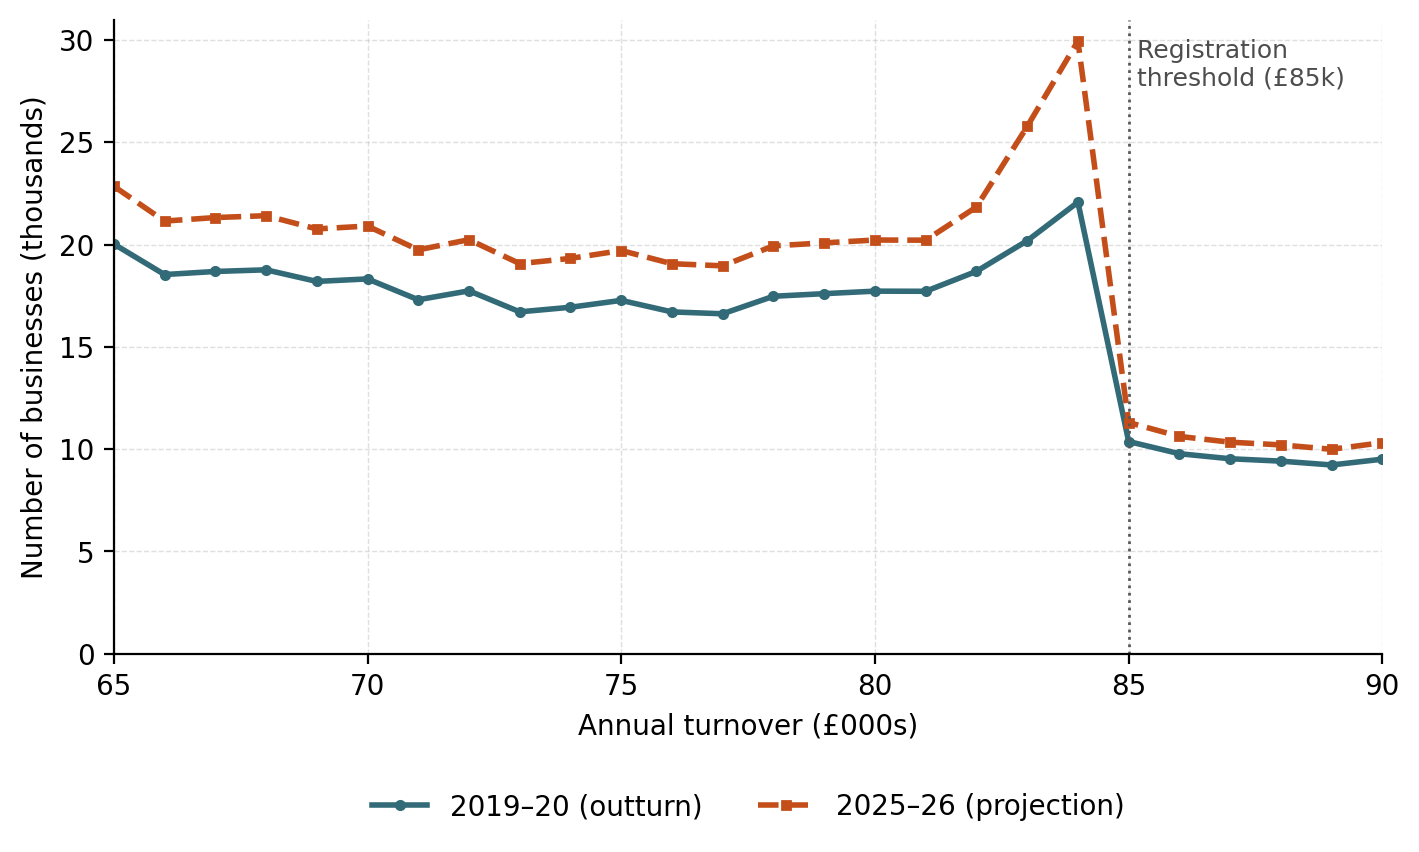
\includegraphics[width=0.74\textwidth]{figures/obr_vat_bunching_85k.png}
\caption{Bunching below the \pounds85{,}000 VAT registration threshold: number of
businesses by \pounds1{,}000 turnover band. Source:
\href{https://obr.uk/box/the-impact-of-the-frozen-vat-registration-threshold/}{OBR,
\emph{Economic and Fiscal Outlook} March 2023}, Chart C (Open Government Licence).}
\label{fig:obr_bunching}
\end{figure}

\paragraph{The reform debate.} The UK threshold is the highest in the OECD
alongside Switzerland \citep{hmrc_threshold},
and there is debate over whether to raise it---to reduce the compliance burden on
small firms---or lower it, to broaden the base and reduce the growth distortion at
the margin. Three families of reform feature, and I evaluate all three: a change in
the threshold's \emph{level} (the \pounds85{,}000 to \pounds90{,}000 increase
of April~2024 and further moves around it); a change in its \emph{shape} (a
\emph{graduated taper} that phases the effective rate in over a band, replacing the
notch with a continuous profile); and a change in its \emph{rate} (a \emph{reduced
rate} for small firms in a band above the threshold, with the standard 20\% rate
retained above). The taper and reduced-rate designs follow proposals in the UK
policy debate: \citet{ots2017vat} canvassed a financial incentive or reduced
effective rate to smooth the cliff-edge at the threshold, and HM Treasury's
call for evidence on the registration threshold examined smoothing mechanisms
in the same family \citep{hmt2018cfe}. The European Union ran a closely
related ``graduated relief'' scheme for small enterprises and abolished it
from January~2025 on complexity grounds, in favour of a simple exemption with
a transition tolerance \citep{eudirective2020285}---relevant precedent for the
administrability of taper-style designs. A banded reduced rate introduces a
smaller \emph{secondary} notch at the band top, which the continuous taper
avoids. I cost all three by the same machinery in Section~\ref{sec:static}.
